%%%%%%%%%%%%%%%%%%%%%%%%%%%%%%%%%%%%%%%%%%%%%%%%%%%%%%%%%%%%%%%%%%%%%%%%%%%%%%%%
%2345678901234567890123456789012345678901234567890123456789012345678901234567890
%        1         2         3         4         5         6         7         8

\documentclass[letterpaper, 10 pt, conference]{ieeeconf}  % Comment this line out
                                                          % if you need a4paper
%\documentclass[a4paper, 10pt, conference]{ieeeconf}      % Use this line for a4
                                                          % paper

\IEEEoverridecommandlockouts                              % This command is only
                                                          % needed if you want to
                                                          % use the \thanks command
\overrideIEEEmargins
% See the \addtolength command later in the file to balance the column lengths
% on the last page of the document

\usepackage[utf8]{inputenc}
\usepackage[T1]{fontenc}
\usepackage{graphicx} %to insert images
% The following packages can be found on http:\\www.ctan.org
%\usepackage{graphics} % for pdf, bitmapped graphics files
%\usepackage{epsfig} % for postscript graphics files
%\usepackage{mathptmx} % assumes new font selection scheme installed
%\usepackage{mathptmx} % assumes new font selection scheme installed
%\usepackage{amsmath} % assumes amsmath package installed
%\usepackage{amssymb}  % assumes amsmath package installed

\title{\LARGE \bf
Matrix Theory Assignment 1
}

%\author{ \parbox{3 in}{\centering Huibert Kwakernaak*
%         \thanks{*Use the $\backslash$thanks command to put information here}\\
%         Faculty of Electrical Engineering, Mathematics and Computer Science\\
%         University of Twente\\
%         7500 AE Enschede, The Netherlands\\
%         {\tt\small h.kwakernaak@autsubmit.com}}
%         \hspace*{ 0.5 in}
%         \parbox{3 in}{ \centering Pradeep Misra**
%         \thanks{**The footnote marks may be inserted manually}\\
%        Department of Electrical Engineering \\
%         Wright State University\\
%         Dayton, OH 45435, USA\\
%         {\tt\small pmisra@cs.wright.edu}}
%}

\author{Ankur Aditya - EE20RESCH11010}



\begin{document}



\maketitle
\thispagestyle{empty}
\pagestyle{empty}


%%%%%%%%%%%%%%%%%%%%%%%%%%%%%%%%%%%%%%%%%%%%%%%%%%%%%%%%%%%%%%%%%%%%%%%%%%%%%%%%
\begin{abstract}

This document contains the procedure to get image of a point in a line. 

\end{abstract}
\\
Download the python code from the below link. Go through the README file in the reposotory.
%
\begin{lstlisting}
https://github.com/ankuraditya13/EE5609-Assignment-1
\end{lstlisting}
%
\\
\begin{comment}
and latex-tikz codes from 
%
\begin{lstlisting}
https://github.com/ankuraditya13/EE5609-Assignment-1
\end{lstlisting}
%
\end{comment}
\section{Problem}

%%%%%%%%%%%%%%%%%%%%%%%%%%%%%%%%%%%%%%%%%%%%%%%%%%%%%%%%%%%%%%%%%%%%%%%%%%%%%%%%
Find the image of the point \left( \begin{array}{c} 3\\ 8\\\end{array}\right) with respect to the line 

   \begin{equation}
         (1\;\;3)\textbf{x} = 7 
\end{equation}       

\section{Solution}


For this problem, I am considering the general case. Let the Equation of line be a*x + b*y = c and let the coordinates of, \\
P(given point) be (x1, y1) \\
Q(image point) be (x2, y2) \\
R(point on mirror) be (x3, y3) \\
\\
Let the slope of perpendicular lines be m1, m2. Hence, 
\begin{equation}
    m1*m2=-1. 
\end{equation}

Now, m1 = \(\frac{y2 - y1}{x2 - x1}\) and m2 = \(\frac{-a}{b}\)\\     \\                                 
Hence upon substituting the value of m1 and m2 in Equation 2 we get,

\begin{equation}
    a*y2 - b*x2 = a*y1 - b*x1
\end{equation}


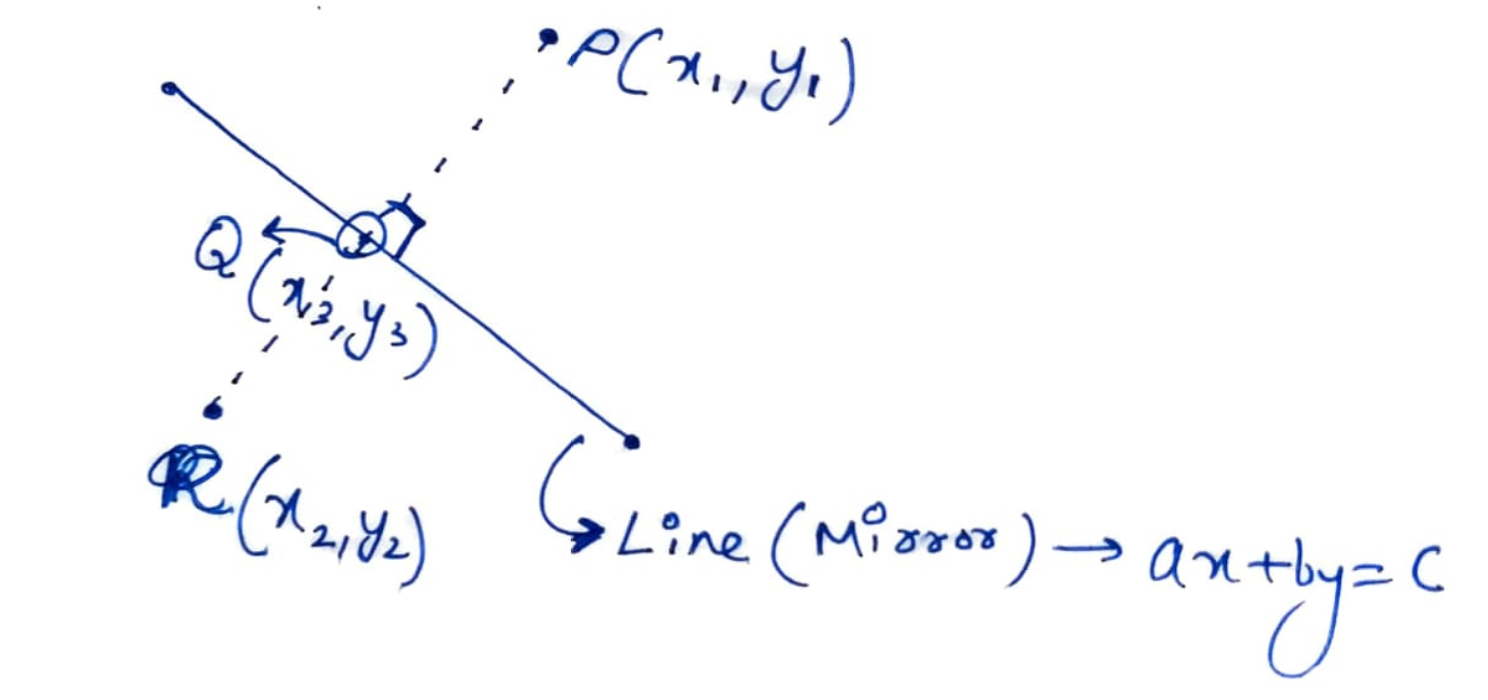
\includegraphics[scale=0.3]{fig1.png} \\


By property in Figure 1, the line PR bisects the mirror equation perpendicularly. Hence, PQ = QR.\\ \\
%\( \frac{1}{2} \)
Hence, x3 = \(\frac{(x1 + x2)}{2}\) and y3 = \(\frac{(y1 + y2)}{2}\) 
Now, clearly from the Figure 1, point Q lies on the line equation a*x + b*y = c. Hence substituting the point Q(x3,y3) in the line equation we get,
\begin{equation}
     b*y2 + a*x2 = -b*y1 - a*x1 + 2*c
\end{equation}
 Solving equation (1) and (2) for x2 and y2 we get,
 
 \begin{equation}
     \[ x2=\frac{2*a*c - 2*a*b*y1 - x1*(a^2 - b^2)}{a^2 + b^2}  
      \end{equation}
     \begin{equation}
         
    
  \[ y2=\frac{2*b*c - 2*a*b*x1 + y1*(a^2 - b^2)}{a^2 + b^2} \ 
 \end{equation}
     
 Hence, substituting the value of x1 = 3, y1 = 8, a = 1, b = 3 and c = 7 in equations (5) and (6) we get,
 \begin{equation}
     x2 = -1
     \end{equation}
     \begin{equation}
         y2 = -4
     \end{equation}
     
 
  Hence, it is the required answer for image of P in line \\(1 3) x =7.
 











\end{document}
